\chapter{Stabilization}
In this section the idea is to stabilize the pendulum in the unstable equilibrium. Ultimately this controller should be able to take over from the swing-up controller when some minimum catch angle is reached.\\
A sliding mode control strategy is employed to accomplish these goals. The design is based on \cite{HKKhalil}.\\
Firstly, the model of the system, from \autoref{eq:nonlinearStateSpace}, is considered in following form,
\begin{align}
  \begin{bmatrix}
    \dot{x_1} \\
    \dot{x_2} \\
    \dot{x_3} \\
    \dot{x_4}
  \end{bmatrix}
  &=
  \underbrace{
    \left[
      \begin{array}{c}
        x_3 \\
        x_4 \\
        \multirow{2}{*}{$ \vec{M}^{-1}(x_1) ( - \vec{C}(x_1,x_3) - \vec{B}(x_3,x_4) - \vec{G}(x_1) ) $}\\
        \phantom{eq}
      \end{array}
    \right]
  }_{\vec{f}(\vec{x})}
  +
  \underbrace{
    \left[
      \begin{array}{c}
        0 \\
        0 \\
        \multirow{2}{*}{$ \vec{M}^{-1}(x_1) \vec{F} $}\\
        \phantom{eq}
      \end{array}
    \right]
  }_{\vec{g}(\vec{x}) u}
\label{eq:nonlinearStateSpace2} \ \ \ ,
\end{align}
%
where,
\begin{align}
  \vec{M}^{-1}
  &=
  \begin{bmatrix}
    \frac{(M + m)}{l^2 m ( M + m - m \cos^2 x_1 )}  &  \frac{\cos x_1}{l (M + m - m \cos^2 x_1)} \\
    \frac{\cos x_1}{l (M + m - m \cos^2 x_1)}       &  \frac{1}{M + m - m \cos^2 x_1}
  \end{bmatrix}  \ \ \ ,
\end{align}
%
with states $ [\ x_1\ \ x_2\ \ x_3\ \ x_4\ ]^\mathrm{T} = [\ \theta\ \ x\ \ \dot{\theta}\ \ \dot{x}\ ]^\mathrm{T} $ and input vector $\vec{F} = [\ 0 \ \ u \ ]^\mathrm{T}$ as before.

In \autoref{eq:nonlinearStateSpace2} the input, $u$, appear in two of the four state equations. To design a sliding mode controller for the system, it is transformed into \textit{regular form}, 
\begin{align}
  \dot{\vec{\eta}} &=  \vec{f_a}(\vec{\eta},\xi) \nonumber   \\
  \dot{\xi}        &=  f_b(\vec{\eta},\xi) + g_b(\vec{\eta},\xi) u    \ \ \ ,
  \label{eq:regularForm}
\end{align}
%
where the input only appears on one state equation.
The transform is then given by,
\begin{align}
  \vec{T}(\vec{x}) &=
  \begin{bmatrix}
    \vec{\eta} \\
    \xi
  \end{bmatrix}
  \ \Rightarrow \ 
  \frac{\partial}{\partial t}\vec{T}(\vec{x})
  =
  \begin{bmatrix}
    \dot{\vec{\eta}} \\
    \dot{\xi}
  \end{bmatrix}
  \ \Rightarrow \ 
  \frac{\partial}{\partial t}\vec{T}(\vec{x})
  =
  \begin{bmatrix}
    \vec{f_a}(\vec{\eta},\xi)         \\
    f_b(\vec{\eta},\xi) + g_b(\vec{\eta},\xi) u
  \end{bmatrix}
   \ \ \ ,
  \label{eq:transformAndDerivative}
\end{align}
further,
\begin{align}
  \frac{\partial \vec{T}}{\partial t} &= \frac{\partial \vec{T}}{\partial \vec{x}}  \dot{\vec{x}} \\
  \begin{bmatrix}
    \vec{f_a}(\vec{\eta},\xi)         \\
    f_b(\vec{\eta},\xi) + g_b(\vec{\eta},\xi) u
  \end{bmatrix}
  &=
  \frac{\partial \vec{T}}{\partial \vec{x}} \vec{f}(\vec{x}) + \frac{\partial \vec{T}}{\partial \vec{x}} \vec{g}(\vec{x}) u
  \ \ \ ,
  \label{eq:transformDerivative}
\end{align}
such that,
\begin{align}
  \frac{\partial \vec{T}}{\partial \vec{x}} \vec{f}(\vec{x})    
  &= 
  \begin{bmatrix}
    \vec{f_a}(\vec{\eta},\xi)       \\
    f_b(\vec{\eta},\xi)
  \end{bmatrix}  \ \ \ \ ,\ \ \ \ 
  \frac{\partial \vec{T}}{\partial \vec{x}} \vec{g}(\vec{x})
  = 
  \begin{bmatrix}
    \vec{0}        \\
    g_b(\vec{\eta},\xi)
  \end{bmatrix}
  \ \ \ .
  \label{eq:transformXDerivative}
\end{align}
\autoref{eq:transformXDerivative} results in the following four equations,
\begin{align}
    \frac{\partial \eta_1}{\partial x_3} g_3 + \frac{\partial \eta_1}{\partial x_4} g_4 &= 0                    \ \ \ \ ,\ \ \ \ % \label{eq:chooseEta1}  \\
    \frac{\partial \eta_2}{\partial x_3} g_3 + \frac{\partial \eta_2}{\partial x_4} g_4 = 0         \nonumber   \\ %\label{eq:chooseEta1Eta2}  \\
    \frac{\partial \eta_3}{\partial x_3} g_3 + \frac{\partial \eta_3}{\partial x_4} g_4 &= 0                    \ \ \ \ ,\ \ \ \ %\label{eq:chooseEta3}  \\
    \frac{\partial \xi   }{\partial x_3} g_3 + \frac{\partial \xi   }{\partial x_4} g_4 = g_b(\vec{\eta},\xi)  \label{eq:chooseEta1Eta2Eta3Xi} 
\ \ \ ,
\end{align}
where,
\begin{align}
  \begin{bmatrix}
    g_3  \\
    g_4
  \end{bmatrix} u = \vec{M}^{-1}(x_1) 
    \begin{bmatrix}
      0  \\
      u
    \end{bmatrix} \ \ \ \Rightarrow \ \ \ \ 
  \begin{cases}
    g_3 = \frac{\cos x_1}{l (M + m - m \cos^2 x1)}\\
    g_4 = \frac{1}{M + m - m \cos^2 x_1 } \ \ \ \ .
  \end{cases}
  \label{eq:g_3_and_4} 
\end{align}
%
The following choice of coordinates to satisfy \autoref{eq:chooseEta1Eta2Eta3Xi} without loss of rank in $\vec{T}$, is based on the transform used for input-output linearization in \cite{HKKhalil}.\\
Choosing output, $h(x) = \theta$ or $h(x) = x$, both results in the relative degree, $\rho = 2$, since the output appears on the second derivatives,
\begin{align}
  \ddot{\theta} &= \dot{x}_3 = f_3 + g_3 u
  \label{eq:thetaRelativeDeg} \\
  \ddot{x} &= \dot{x}_4 = f_4 + g_4 u \ \ \ .
  \label{eq:xRelativeDeg} 
\end{align}
The suggested transform is then,
\begin{align}
  \vec{T}(\vec{x})
  =
  \begin{bmatrix}
    \phi_1(\vec{x})         \\
    \vdots                  \\
    \phi_{n-\rho}(\vec{x})  \\
    h(\vec{x})              \\
    L_f h(\vec{x})          \\
    \vdots                  \\
    L_f^{\rho-1} h(\vec{x})
  \end{bmatrix}
  \ \ \Rightarrow \ \ 
  \begin{bmatrix}
    \eta_1   \\
    \eta_2   \\
    \eta_3   \\
    \xi
  \end{bmatrix}
  =
  \begin{bmatrix}
    \phi_1(\vec{x})   \\
    \phi_2(\vec{x})   \\
    h(\vec{x})        \\
    L_f h(\vec{x})
  \end{bmatrix} \ \ \ ,
  \label{eq:transformPhi} 
\end{align}
%
where $L_f h(\vec{x})$ is the \textit{Lie derivative} of $h(\vec{x})$ along $f(\vec{x})$. This results in two possible transforms, 
\begin{align}
h = \theta \ \ \Rightarrow \ \ 
  \vec{T}_1 =
  \begin{bmatrix}
    \eta_1  \\
    \eta_2  \\
    \eta_3  \\
    \xi
  \end{bmatrix}
  =
  \begin{bmatrix}
    \phi_1  \\
    \phi_2  \\
    x_1     \\
    x_3
  \end{bmatrix} \ \ \ \mathrm{and}\ \ h = x \ \ \Rightarrow \ \
  \vec{T}_2 =
  \begin{bmatrix}
    \eta_1   \\
    \eta_2   \\
    \eta_3   \\
    \xi
  \end{bmatrix}
  =
  \begin{bmatrix}
    \phi_1  \\
    \phi_2  \\
    x_2     \\
    x_4
  \end{bmatrix} \ \ \ ,
\end{align}
leaving $\phi_1$ and $\phi_2$ to be determined. This is done by satisfying,
\begin{align}
  \frac{\partial \eta_1}{\partial x_3} g_3 + \frac{\partial \eta_1}{\partial x_4} g_4 &= 0       \label{eq:chooseEta1}  \\
  \frac{\partial \eta_2}{\partial x_3} g_3 + \frac{\partial \eta_2}{\partial x_4} g_4 &= 0       \label{eq:chooseEta2}  
  \ \ \ ,
\end{align}
from \autoref{eq:chooseEta1Eta2Eta3Xi}. For $\vec{T}_1$ the choice $\phi_1 = x_2$ satisfies \autoref{eq:chooseEta1} with no loss of rank in the transform. Conversely for $\vec{T}_2$ the choice $\phi_1 = x_1$ satisfies \autoref{eq:chooseEta1} again with no loss of rank. This leaves $\phi_2$ which, for both transforms, is determined by finding a solution to \autoref{eq:chooseEta2},
\begin{align}
  \frac{\partial \eta_2}{\partial x_3} \frac{\cos x_1}{l (M + m - m \cos^2 x1)} + \frac{\partial \eta_2}{\partial x_4} \frac{1}{M + m - m \cos^2 x_1 } = 0 \ \ \ ,
\end{align}
choosing,
\begin{align}
  \frac{\partial \eta_2}{\partial x_4} = \frac{\cos x_1}{l}  \ \ , \ \ \ \frac{\partial \eta_2}{\partial x_3}  = -1 \ \ \ ,
\end{align}
such that,
\begin{align}
  \eta_2 =  \frac{\cos x_1}{l} x_4 - x_3 \ \ \ .
\end{align}
%
This results in the following two transform candidates,
\begin{align}
  %\begin{bmatrix}
  %\eta_1   \\
  %\eta_2   \\
  %\eta_3   \\
  %\xi
  %\end{bmatrix} \left.\rule{0cm}{1.7cm}\right\vert\rule{0cm}{1.7cm}_{\substack{\rule{0cm}{1.28cm}\\ h=x_1 }}
  \vec{T}_1 =
  \begin{bmatrix}
    x_2   \\
    \frac{\cos x_1}{l} x_4 - x_3  \\
    x_1   \\
    x_3
  \end{bmatrix} \ \ \ \ , \ \ \ \
  %\begin{bmatrix}
  %\eta_1   \\
  %\eta_2   \\
  %\eta_3   \\
  %\xi
  %\end{bmatrix} \left.\rule{0cm}{1.7cm}\right\vert\rule{0cm}{1.7cm}_{\substack{\rule{0cm}{1.28cm}\\ h=x_2 }}
  \vec{T}_2
  =
  \begin{bmatrix}
    x_1   \\
    \frac{\cos x_1}{l} x_4 - x_3   \\
    x_2   \\
    x_4
  \end{bmatrix} \ \ \ .
\end{align}
%
%To choose a transform the following is considered.\\
It is desired for the transform, $\vec{T}$, to be continuously differentiable and have a continuously differentiable inverse, $\vec{T}^{-1}$. Such a transform is known as a diffeomorphism. Further, $\vec{T}$ is a global diffeomorphism iff its Jacobian is nonsingular for all $\vec{x} \in \mathbb{R}^n$ and $\lim_{||\vec{x}||\rightarrow \infty}||\vec{T}(\vec{x})|| = \infty$ , \cite{HKKhalil}.\\
Thus the Jacobian of each transform is computed,
\begin{align}
  \vec{J}_1 = \frac{\partial \vec{T}_1(\vec{x})}{\partial \vec{x}}
  &=
  \begin{bmatrix}
    0                       & 1 &  0 & 0                  \\
    -\frac{\sin x_1}{l} x_4 & 0 & -1 & \frac{\cos x_1}{l} \\
    1                       & 0 &  0 & 0                  \\
    0                       & 0 &  1 & 0
  \end{bmatrix}  \label{eq:transform_h_x1} \\
  \vec{J}_2 = \frac{\partial \vec{T}_2(\vec{x})}{\partial \vec{x}}
  &=
  \begin{bmatrix}
    1                       & 0 &  0 & 0                  \\
    -\frac{\sin x_1}{l} x_4 & 0 & -1 & \frac{\cos x_1}{l} \\
    0                       & 1 &  0 & 0                  \\
    0                       & 0 &  0 & 1
  \end{bmatrix} \ \ \ . \label{eq:transform_h_x2}
\end{align}
To check for singularity the determinant is found for the two Jacobian matrices,
\begin{align}
  \det(\vec{J}_1) &= -\frac{\cos x_1}{l} \ \ \ \ , \ \ \ \  \det(\vec{J}_2) = 1 \ \ \ . \label{eq:determinantOfJ1andJ2}
\end{align}
If $\cos x_1 = 0$ the Jacobian, $\vec{J}_1$, becomes singular. This only happens when the pendulum is in a horizontal position, which is outside the operating range of a stabilizing controller. However, the Jacobian, $\vec{J}_2$, is nonsingular for all $\vec{x} \in \mathbb{R}^4$. Further, $\lim_{||\vec{x}||\rightarrow \infty}||\vec{T}_2(\vec{x})|| = \infty$ so,
\begin{align}
  \vec{T}
  = 
  \begin{bmatrix}
    \eta_1   \\
    \eta_2   \\
    \eta_3   \\
    \xi
  \end{bmatrix}
  =
  \begin{bmatrix}
    x_1   \\
    \frac{\cos x_1}{l} x_4 - x_3  \\
    x_2   \\
    x_4
  \end{bmatrix} \ \ \ , \label{eq:transform}
\end{align}
is a global diffeomorphism and therefore chosen as the final system transform, with the inverse given by,
\begin{align}
  \vec{T}^{-1} = 
  \begin{bmatrix}
    x_1  \\
    x_2  \\
    x_3  \\
    x_4
  \end{bmatrix}
  =
  \begin{bmatrix}
  \eta_1   \\
  \eta_3   \\
  \frac{\cos \eta_1}{l} \xi - \eta_2  \\
  \xi
  \end{bmatrix} \ \ \ .
  \label{eq:inverseTransform}
\end{align}
%
The derivative of the transform, \autoref{eq:transform}, along the trajectories of the system is,
\begin{align}
  \begin{bmatrix}
    \dot{\eta}_1   \\
    \dot{\eta}_2   \\
    \dot{\eta}_3   \\
    \dot{\xi}
  \end{bmatrix}
  &=
  \begin{bmatrix}
    \dot{x}_1   \\
    \frac{-\sin x_1}{l}\dot{x}_1 x_4 + \frac{\cos x_1}{l} \dot{x}_4 - \dot{x}_3  \\
    \dot{x}_2   \\
    \dot{x}_4
  \end{bmatrix} \label{eq:transform_dt} \\
  %
  %
  %
  \begin{bmatrix}
  \dot{\eta}_1   \\
  \dot{\eta}_2   \\
  \dot{\eta}_3   \\
  \dot{\xi}
  \end{bmatrix} 
  &=
  \begin{bmatrix}
    x_3    \\
    \frac{-\sin x_1}{l} x_3 x_4 + \frac{\cos x_1}{l} f_4(\vec{x}) + \frac{\cos x_1}{l} g_4(\vec{x}) u  - f_3(\vec{x}) - g_3(\vec{x}) u \\
    x_4    \\ 
    f_4(\vec{x}) + g_4(\vec{x}) u 
  \end{bmatrix} \ \ \ , \label{eq:transform_dt_alongTraj}
\end{align}
%
from which the \textit{regular form} is obtained by rearranging and using the inverse transform,
\begin{align}
  \begin{bmatrix}
    \dot{\eta}_1   \\
    \dot{\eta}_2   \\
    \dot{\eta}_3   \\  %these are dotted lines, yea, that's LaTeX for ya, go figure..
    %\begin{picture} (0,0)(0,0) \multiput(-2,14)(4,0){3}{\line(2,0){2}} \end{picture}
    \dot{\xi}
  \end{bmatrix} 
  &=
  \begin{bmatrix}
    \multirow{3}{*}{$ \vec{f_a}(\vec{\eta},\phi(\vec{\eta})) $}\\
    \\
    \\
    \begin{picture} (0,0)(0,0) \multiput(.5,14)(4,0){14}{\line(2,0){2}} \end{picture}
     f_b(\vec{\eta},\phi(\vec{\eta}))
  \end{bmatrix}
  +
  \begin{bmatrix}
    0 \\
    0 \\
    0 \\
    \begin{picture} (0,0)(0,0) \multiput(-0,14)(4,0){14}{\line(2,0){2}} \end{picture}
    g_b(\vec{\eta},\phi(\vec{\eta})) 
  \end{bmatrix} \\
%
%
  \begin{bmatrix}
    \dot{\eta}_1   \\
    \dot{\eta}_2   \\
    \dot{\eta}_3   \\  %these are dotted lines, yea, that's LaTeX for ya, go figure..
    %\begin{picture} (0,0)(0,0) \multiput(-2,14)(4,0){3}{\line(2,0){2}} \end{picture}
    \dot{\xi}
  \end{bmatrix} 
  &=
  \begin{bmatrix}
    \frac{\cos \eta_1}{l} \xi - \eta_2    \\
    %\frac{l \sin x1}{\cos^2 x_1} x_3^2 +  \tfrac{l}{\cos x_1} f_1(\vec{x})  - f_2(\vec{x}) \\ 
    \frac{-\sin \eta_1}{l} (\frac{\cos \eta_1}{l} \xi - \eta_2) \xi + \frac{\cos \eta_1}{l} f_4(\vec{\eta},\xi) - f_3(\vec{\eta},\xi) \\
    \xi    \\ %these are dotted lines, yea, that's LaTeX for ya, go figure..
    \begin{picture} (0,0)(0,0) \multiput(-95,14)(4,0){57}{\line(2,0){2}} \end{picture}
    f_4(\vec{\eta},\xi) 
  \end{bmatrix}
  \begin{bmatrix}
    0    \\
    0    \\
    0    \\  %these are dotted lines, yea, that's LaTeX for ya, go figure..
    \begin{picture} (0,0)(0,0) \multiput(0,14)(4,0){10}{\line(2,0){2}} \end{picture}
    g_4(\vec{\eta},\xi)
  \end{bmatrix}
  \ \ \ ,
  \label{eq:regularFormMatrix}
\end{align}
where,
\begingroup\makeatletter\def\f@size{10}\check@mathfonts
\def\maketag@@@#1{\hbox{\m@th\normalsize\normalfont#1}}%
\begin{align}
f_3(\vec{\eta},\xi) &= \frac{1}{ l^2 m (M + m - m \cos^2 \eta_1) }
\left[
(M + m) b_{p,v} \left(\eta_2 - \frac{\cos \eta_1 \xi}{l}\right) + \right. \nonumber \\
&+ (M + m) b_{p,c} \tanh\left(\mathrm{k}_{\mathrm{tanh}} \left(\eta_2 - \frac{ \cos \eta_1 \xi}{l}\right)\right) + m^2 g l \sin \eta_1 - b_{c,c} m l \tanh\left(\mathrm{k}_{\mathrm{tanh}} \xi\right) \cos \eta_1 - \nonumber \\
&- \left. m^2 l^2 \cos \eta_1 \sin \eta_1 \left(\eta_2 - \frac{\xi \cos \eta_1}{l}\right)^2 + M g l m \sin \eta_1 - b_{c,v} m l \xi \cos \eta_1
\right] \\
%
%
f_4(\vec{\eta},\xi) &= -\frac{1}{ l (M + m - m \cos^2 \eta_1) } \left[   b_{c,v} l \xi - b_{p,v} \cos \eta_1 \left(\eta_2 - \frac{\cos \eta_1 \xi}{l}\right) + b_{c,c} l \tanh\left(\mathrm{k}_{\mathrm{tanh}} \xi\right) - \right. \nonumber \\
&- b_{p,c} \tanh\left(\mathrm{k}_{\mathrm{tanh}} \left(\eta_2 - \frac{ \cos \eta_1 \xi}{l}\right)\right) \cos \eta_1 + \nonumber \\
&+ \left. l^2 m \sin \eta_1 \left(\eta_2 - \frac{\xi \cos \eta_1}{l}\right)^2 - m g l \cos \eta_1 \sin \eta_1  \right] \\
%
%
g_4(\vec{\eta},\xi) &= \frac{1}{M + m - m \cos^2 \eta_1 }
\ \ \ .
\label{eq:f3f4g4} \\ \nonumber
\end{align}
\endgroup \vspace{-44pt}

%
%
%
%f3 = \frac{ M b_{p,v} (\eta_2 - \frac{\xi \cos \eta_1}{l}) + b_{p,v} m (\eta_2 - \frac{\xi \cos \eta_1}{l}) + M b_{p,c} \tanh(k_{\mathrm{tanh}} (\eta_2 - \frac{\xi \cos \eta_1}{l})) + b_{p,c} m \tanh(k_{\mathrm{tanh}} (\eta_2 - \frac{\xi \cos \eta_1}{l})) + g l m^2 \sin \eta_1 - b_{c,c} l m \tanh(k_{\mathrm{tanh}} \xi) \cos \eta_1 - l^2 m^2 \cos \eta_1 \sin \eta_1 (\eta_2 - \frac{\xi \cos \eta_1}{l})^2 + M g l m \sin \eta_1 - b_{c,v} l m \xi \cos \eta_1 }{ l^2 m (M + m - m \cos^2 \eta_1) }
%
%
%
%f4 = -\frac{1}{ l (M + m - m \cos^2 \eta_1) } \left[   b_{c,v} l \xi - b_{p,v} \cos \eta_1 \left(\eta_2 - \frac{\cos \eta_1 \xi}{l}\right) + b_{c,c} l \tanh\left(\mathrm{k}_{\mathrm{tanh}} \xi\right) - b_{p,c} \tanh\left(\mathrm{k}_{\mathrm{tanh}} \left(\eta_2 - \frac{ \cos \eta_1 \xi}{l}\right)\right) \cos \eta_1 + l^2 m \sin \eta_1 \left(\eta_2 - \frac{\xi \cos \eta_1}{l}\right)^2 - m g l \cos \eta_1 \sin \eta_1  \right]
%
%
%
%
With the system on regular form, design is proceeded by choosing a sliding manifold,
\begin{align}
s &=   \xi - \phi(\vec{\eta})    \ \ \ ,
\end{align}
where $\phi(\vec{\eta})$ is to be designed. If $s$ is zero then $\xi = \phi(\vec{\eta})$, such that,
\begin{align}
\vec{\dot{\eta}} &=  f_a(\vec{\eta},\phi(\vec{\eta}))     \ \ \ ,
\label{eq:reducedOrderSys}
\end{align}
is the reduced-order system with $\phi(\vec{\eta})$ as control input. It is then sought to design $\phi(\vec{\eta})$ such that \autoref{eq:reducedOrderSys} is asymptotically stable at its origin.\\
To that end, the reduced-order system is linearized,
%
\begin{align}
  A &= \frac{\partial \vec{\dot{\eta}}}{\partial \vec{\eta}} \whereThree{\vec{\eta}=\vec{0}\ \ \ \ }{\xi=0\ \ \ \ }{\text{k}_\text{tanh}=1} \ 
  =
  \begin{bmatrix}
    0           & -1                     & 0 \\
   -\frac{g}{l} & \frac{-b_{p,v}}{l^2 m} & 0 \\
    0           & 0                      & 0 
  \end{bmatrix}   \ \ \ , \ \ \
  B = \frac{\partial \vec{\dot{\eta}}}{\partial \xi} \whereThree{\vec{\eta}=\vec{0}\ \ \ \ }{\xi=0\ \ \ \ }{\text{k}_\text{tanh}=1} \ 
  =
  \begin{bmatrix}
    \frac{1}{l}                       \\
    \frac{b_{p,v} + b_{p,c} l}{l^3 m} \\
    1 
  \end{bmatrix}   \ \ \ .
  \label{eq:linearReducedOrder_A}
\end{align}
%
Checking for controllability,
\begin{align}
  \mathrm{rank}(\mathcal{C}) &= \mathrm{rank}([\ \begin{matrix} B & AB & A^2 B \end{matrix}\ ]) = 3  \ \ \ ,
\end{align}
and since the controllability matrix, $\mathcal{C}$, has full rank, the linearized system is controllable.
%
A state feedback controller is designed for the linearized reduced-order system,
\begin{align}
\phi(\vec{\eta}) &=   - \vec{k} \vec{\eta}  \ \ \ .
\end{align}
%
The poles are placed in $\vec{p} = [\ \ -4 \ -6 \ -7\ \ ]$ using matlab \textit{place()}-command to obtain the gains, $\vec{k} =  [\ \ 7.2025 \ -1.2930 \ -5.4218 \ \ ]$. Simulations of the controlled reduced-order system are run for both the linearized and the nonlinear system, see \autoref{fig:reducedOrderControlledSimulation}.
%
\begin{figure}[H]
  \captionsetup[subfigure]
  {
    margin          = {12pt,5pt}  %caption margin
  }
  \subcaptionbox{The angle reaches zero with small oscillations in the nonlinear simulation.}[0.4\textwidth] %caption width
  {
    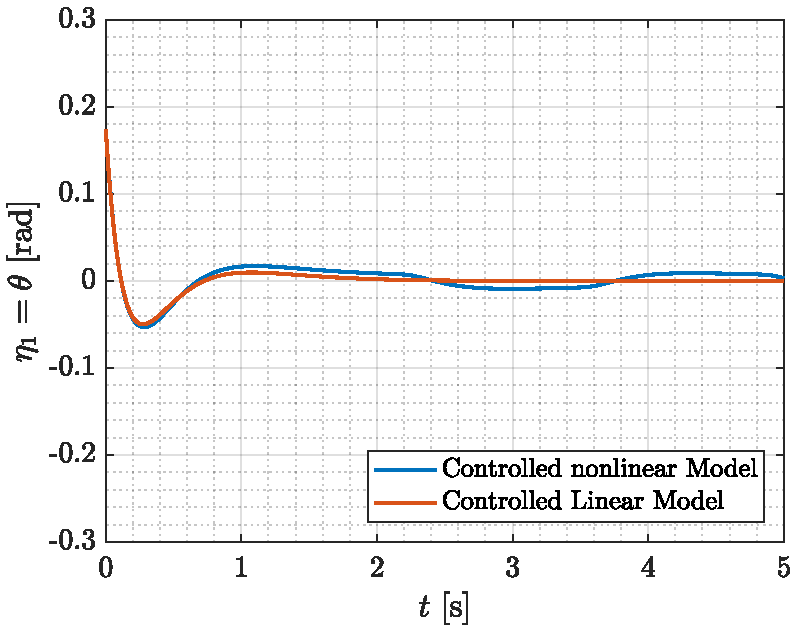
\includegraphics[width=0.4\textwidth]{figures/eta1}
  }
  \hspace{.5cm}
  \subcaptionbox{Large oscillations occur in the nonlinear simulation. This parameter does not directly have a physical interpretation.}[0.4\textwidth] %caption width
  {
    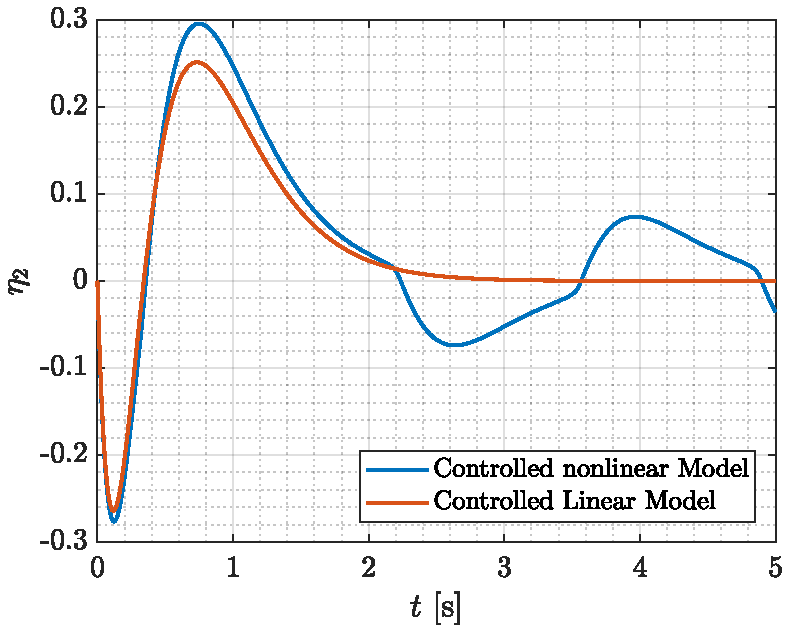
\includegraphics[width=0.4\textwidth]{figures/eta2}
  }

  \subcaptionbox{The cart position reaches zero with small oscillations in the nonlinear simulation.}[0.4\textwidth] %caption width
  {
    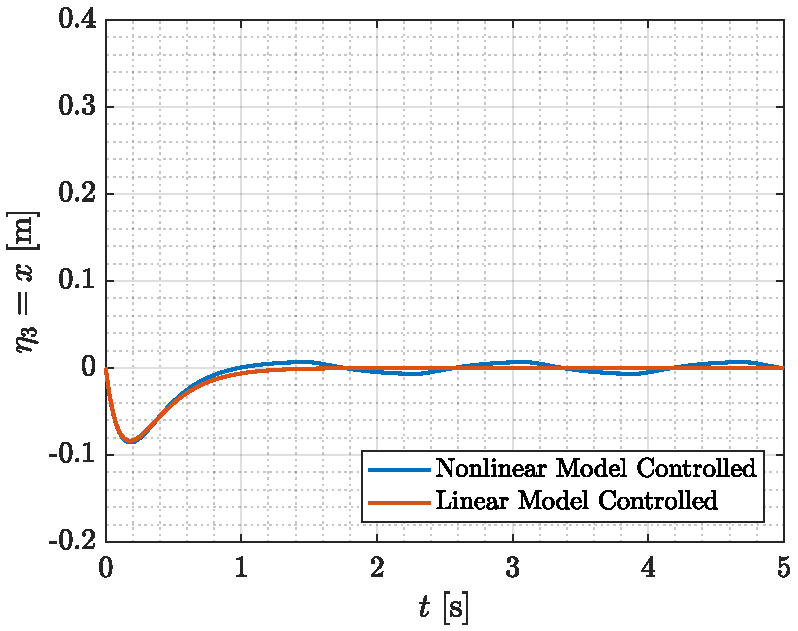
\includegraphics[width=0.4\textwidth]{figures/eta3}
  }
  \hspace{.5cm}
  \subcaptionbox{The tendency to oscillations in the nonlinear simulation also appears in the control signal for the reduced-order system.}[0.4\textwidth] %caption width
  {
    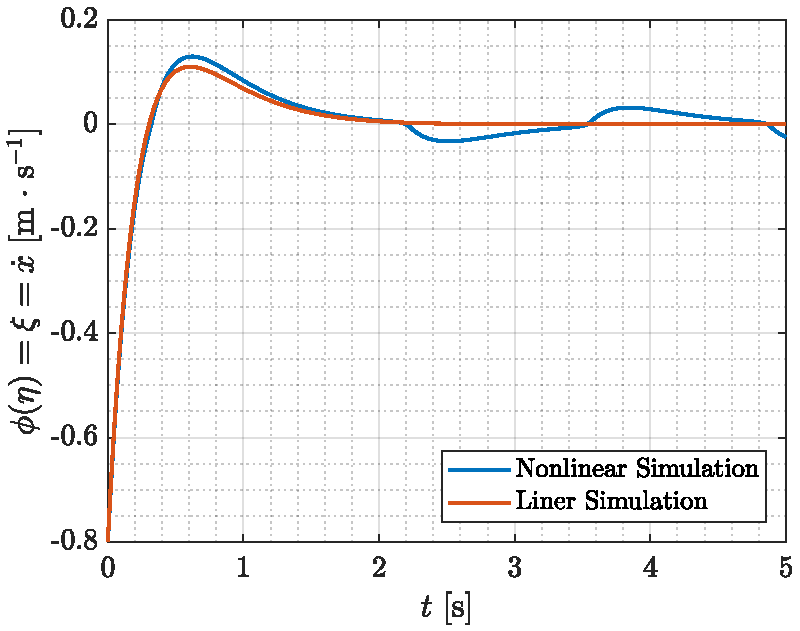
\includegraphics[width=0.4\textwidth]{figures/xi}
  }
  \caption{Nonlinear and linear simulation of the state feedback control designed for the linearized reduced-order system.}
  \label{fig:reducedOrderControlledSimulation}
\end{figure}
%
%
The reduced-order system is stabilized under the assumption that $s$ is zero. Thus, the design of $u$ is concerned with bringing $s$ to zero.

\begin{minipage}{\textwidth}
\begin{theorem}[Lyapunov Stability Theorem]
  \label{th:lyapunovStabilityTheorem}
  Consider the autonomous system, $f(\vec{x}) = \dot{\vec{x}}$, where $f : \mathbb{D} \rightarrow \mathbb{R} ^n$ is locally Lipschitz and $\vec{x}=\vec{0}$ is an equilibrium point. Then if $\exists\ V : \mathbb{D} \rightarrow \mathbb{R}$ and %\vspace{-12pt}
  \begin{enumerate}
    \item $V(\vec{x})$ is $C^1$
    \item $V(\vec{x}) > 0$ $\forall\ \vec{x} \in \mathbb{D}\backslash 0$ and $V(\vec{0}) = 0$
    \item $\dot{V}(\vec{x}) \leq 0$ in $\mathbb{D}$
  \end{enumerate} %\vspace{-12pt}
  then $\vec{x} = \vec{0}$ is stable. Further, if,
  %\vspace{-12pt}
  \begin{itemize}
    \item[] $ \dot{V}(\vec{x}) < 0\ \mathrm{in}\ \mathbb{D}\backslash 0  \ \ \ ,  $
  \end{itemize}%\vspace{-12pt}
  then $\vec{x} = \vec{0}$ is asymptotically stable \cite{HKKhalil}.
\end{theorem}%\vspace{-12pt}
\end{minipage}

A Lyapunov function candidate is proposed,
\begin{align}
  V(\vec{\eta}, \xi) &= \tfrac{1}{2}s^2 \ \ \ , \label{eq:lyapunovFunctionCandidate}
\end{align}
where $s = \xi - \vec{k} \vec{\eta}$ hence,
\begin{align}
V &= \tfrac{1}{2}(\xi - \vec{k} \vec{\eta})^2 \label{eq:lyapunovFC}\\
V &= \tfrac{1}{2}( \xi^2 + (\vec{k} \vec{\eta})^2 ) - \xi \vec{k} \vec{\eta} \\
V &= \tfrac{1}{2}( \xi^2 + k_1^2 \eta_1^2 + k_2^2 \eta_2^2 + k_3^2 \eta_3^2 ) + k_1 k_2 \eta_1 \eta_2 + k_1 k_3 \eta_1 \eta_3 + k_2 k_3 \eta_2 \eta_3 - \nonumber \\
  &- \xi ( k_1 \eta_1 + k_2 \eta_2 + k_3 \eta_3 )
\ \ \ . \label{eq:lyapunovFCExpanded}
\end{align}
The partial derivatives are,
%% derivatives  for eta1 and xi   and if they are C^0  --> V is C^1
\begin{align}
  \frac{\partial V}{\partial \xi}    &= \xi - \vec{k}\vec{\eta}
    \label{eq:lyapunovCandidateDiff_xi} \\
  \frac{\partial V}{\partial \eta_1} &= k_1^2 \eta_1 + k_1 k_2 \eta_2 + k_1 k_3 \eta_3 - k_1 \xi
    \label{eq:lyapunovCandidateDiff_eta1} 
    \ \ \ ,
\end{align}
and similar results to \autoref{eq:lyapunovCandidateDiff_eta1} are obtained for the partial derivatives with respect to $\eta_2$ and $\eta_3$. Since all four partial derivatives are $C^0$ then $V$ is $C^1$ in the entire $\mathbb{R} ^4$, thus satisfying the first condition of the Lyapunov Stability \autoref{th:lyapunovStabilityTheorem}. Further, from \autoref{eq:lyapunovFC}, it is clear that $V$ is positive definite in the entire state space without zero and zero in the origin, thus also satisfying the second condition.\\
To assess the third condition of \autoref{th:lyapunovStabilityTheorem}, the derivative of the Lyapunov function candidate is found along trajectories of the system,
\begin{align}
\dot{V} &= s\dot{s} \\
\dot{V} &= s ( \dot{\xi} + \vec{k}\vec{\dot{\eta}}  ) \\
\dot{V} &= s ( f_b(\vec{\eta},\xi) + g_b(\vec{\eta},\xi) u +\vec{k}f_a(\vec{\eta},\xi) )  \\
\dot{V} &= (\vec{k}f_a +  f_b) s + g_b s u \\
\dot{V} &= g_b s (\vec{k}f_a  +  f_b) g_b^{-1} + g_b s u   \\
\dot{V} &\leq g_b |s| \left|\vec{k}f_a  +  f_b \right| g_b^{-1} + g_b s u  \ \ \ .
\label{eq:lyapunov}
\end{align}
This leads to the design of $u$ which is chosen such that the third condition of \autoref{th:lyapunovStabilityTheorem} is satisfied,
\begin{align}
u = -\text{sgn}(s)\beta (\vec{\eta},\xi) g_b^{-1}(\vec{\eta},\xi) \ \ \ \ \mathrm{where}, \ \ \ \beta(\vec{\eta},\xi)  &= \varrho(\vec{\eta},\xi) + \beta_0 \\
\ \ \ \ \ \ \  \varrho(\vec{\eta},\xi) &= \left|\vec{k}f_a  +  f_b \right| \ \ \ ,
\label{eq:ssControlBeta0}
\end{align}
and  $\beta_0 > 0$ is a tuning parameter allowing $\dot{V}$ to be positive definite, thereby guaranteeing asymptotic stability of the origin by \autoref{th:lyapunovStabilityTheorem},
\begin{align}
\dot{V} &< g_b |s| \left|\vec{k}f_a +  f_b \right|  g_b^{-1} - g_b\  \mathrm{sgn}(s) s \left|\vec{k}f_a  +  f_b + \beta_0 \right| g_b^{-1} \ \ \ .
\label{eq:lyapunov2}
\end{align}
For implementation, the discontinuity introduced by the sign-function in the control law is cause for excessive switching and chattering due to delays in the real system. To circumvent this issue, a saturation function with a steep slope, $1/\varepsilon$, is used to approximate the sign-function,
\begin{align}
\text{sat}\left( s/\varepsilon \right) &=
\begin{cases}
\ \ s/\varepsilon              &  \ | s/\varepsilon | \leq 1 \\
\ \ \text{sgn}\left( s \right) &  \ | s/\varepsilon |  >   1 \ \ \ ,
\end{cases}
\label{eq:satuationFunction2}
\end{align}
hence,
\begin{align}
u &= -\text{sat}(s/\varepsilon)\beta (\vec{\eta},\xi)  g_b^{-1}(\vec{\eta},\xi)  \ \ \ .
\label{eq:ssControlSat}
\end{align}

A simulation of the design is shown in \autoref{fig:theta_slidingMode} and \ref{fig:x_slidingMode}, starting from an initial angle of \SI{0.1}{rad \cdot s^{-1}}. Both the angle and cart position are brought to zero. The small oscillations are thought to origin from the linear part of the design, where oscillations were observed in the simulation of the nonlinear reduced order system with linear control, see \autoref{fig:reducedOrderControlledSimulation}.
%
%AVAILABLE PLOTS FROM THIS SIMULATION
%x_slidingMode
%xDot_slidingMode
%xDotDot_slidingMode
%theta_slidingMode
%thetaDot_slidingMode
%thetaDotDot_slidingMode
%ia_slidingMode
%phase_slidingMode
%Edelta_slidingMode
%ani_slidingMode
\begin{figure}[H]
  \hspace{-10pt}
  \captionbox
  {
    A simulation of the sliding mode design starting form an initial angle of \SI{0.1}{rad \cdot s^{-1}} at zero angular velocity. The angle is maintained around zero with small oscillation.
    \label{fig:theta_slidingMode}
  }
  {
    \hspace{-1cm}
    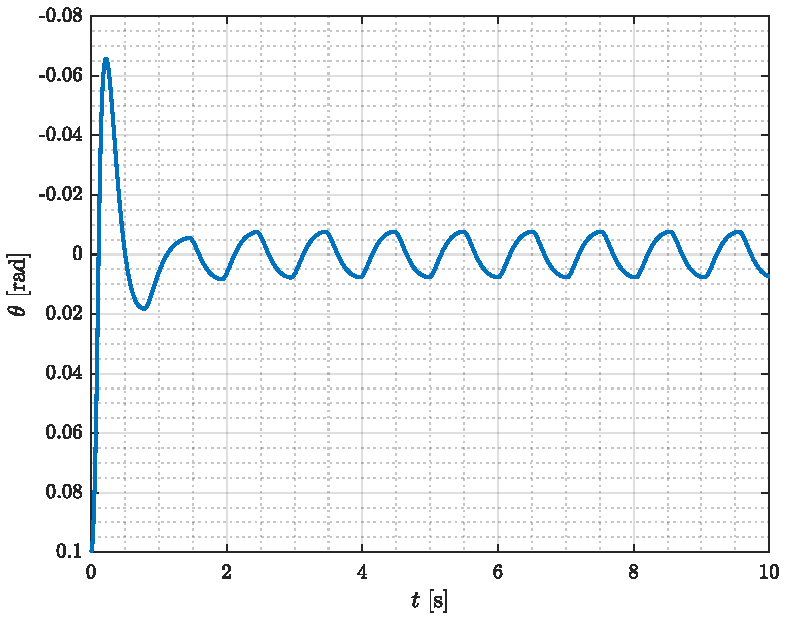
\includegraphics[width=.4\textwidth]{figures/theta_slidingMode}
  }
  \hspace{20pt}
  \captionbox 
  {
    The cart position successfully returns to zero with small oscillations after the pendulum angle is brought to zero.
    \label{fig:x_slidingMode}
  }
  {
    \hspace{-1cm}
    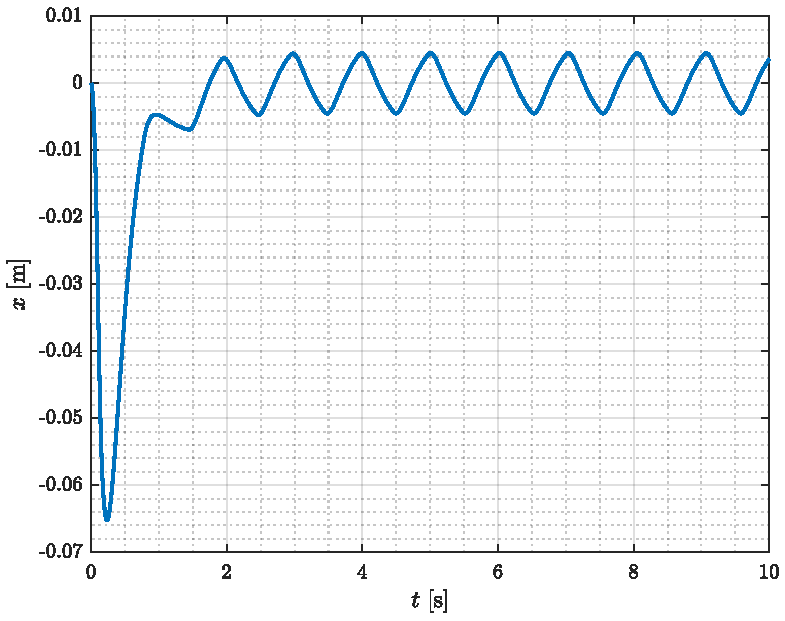
\includegraphics[width=.4\textwidth]{figures/x_slidingMode}
  }  
\end{figure}
%
To achieve this behavior from relatively wide catch angle, a large peak occurs in the armature current, see \autoref{fig:ia_slidingMode}. However, with the short duration of the peak, this is not considered a problem. If it is desired to bring down the peak current, the sliding mode controller could simply be activated at a narrower angle.
%
\begin{figure}[H]
  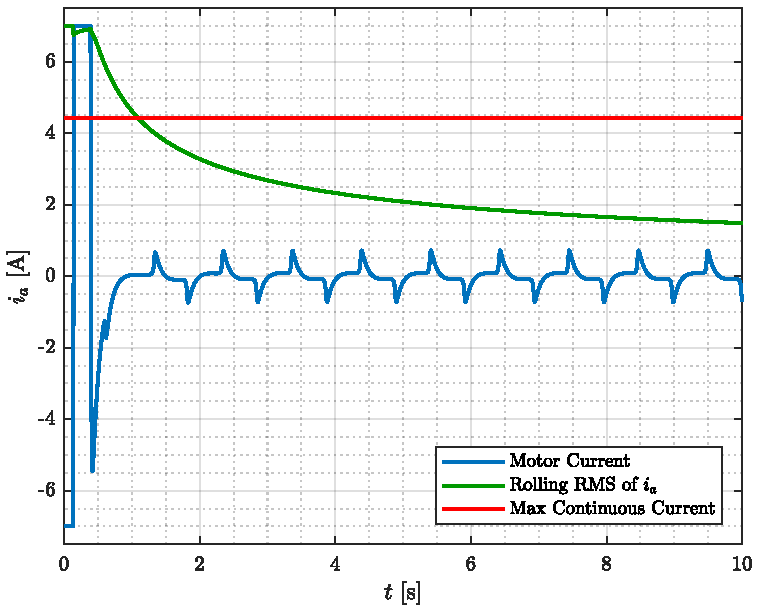
\includegraphics[width=.42\textwidth]{figures/ia_slidingMode}
  \caption{The control signal from the simulation in \autoref{fig:theta_slidingMode} and \ref{fig:x_slidingMode}. The peak current is rather large, which is to be expected given the relatively wide initial angle. It is not considered to be a problem, since the large current is only maintained for a short duration.}
  \label{fig:ia_slidingMode}
\end{figure}
%
Finally the swing-up controller and the sliding mode controller are simulated in concert, where the sliding mode controller is activated at a catch angle of \SI{0.1}{rad}. The result is seen in \autoref{fig:theta_swingAndCatch} and \autoref{fig:x_swingAndCatch}, where the swing-up controller brings the angle below the catch angle in seven swings, after which the system is stabilized in zero by the sliding mode controller.
%
%AVAILABLE PLOTS FROM THIS SIMULATION
%x_swingAndCatch
%xDot_swingAndCatch
%xDotDot_swingAndCatch
%theta_swingAndCatch
%thetaDot_swingAndCatch
%thetaDotDot_swingAndCatch
%ia_swingAndCatch
%phase_swingAndCatch
%Edelta_swingAndCatch
%ani_swingAndCatch
\begin{figure}[H]
  \hspace{-10pt}
  \captionbox
  {
    Simulation of the swing-up controller using sliding mode to catch the pendulum when the angle reaches below \SI{0.1}{rad}.
    \label{fig:theta_swingAndCatch}
  }
  {
    \hspace{-1cm}
    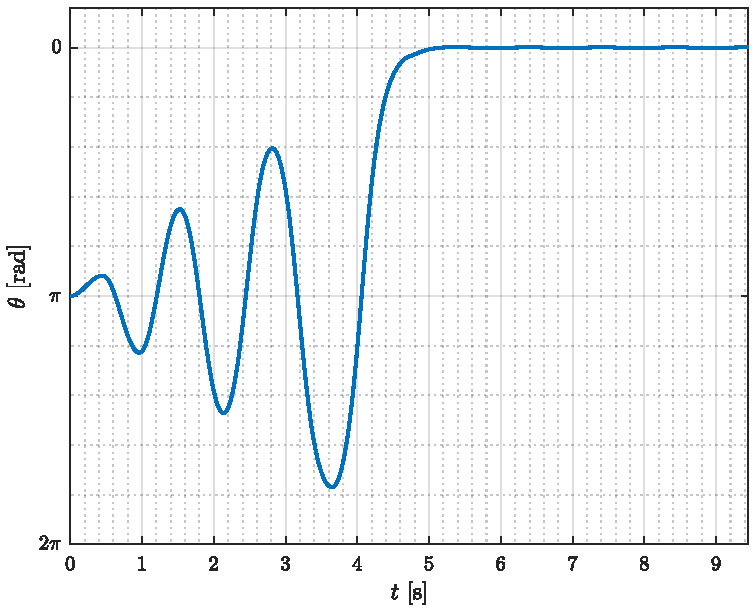
\includegraphics[width=.4\textwidth]{figures/theta_swingAndCatch}
  }
  \hspace{20pt}
  \captionbox 
  {
    The cart position successfully returns to zero after the pendulum angle is stabilized at zero.
    \label{fig:x_swingAndCatch}
  }
  {
    \hspace{-1cm}
    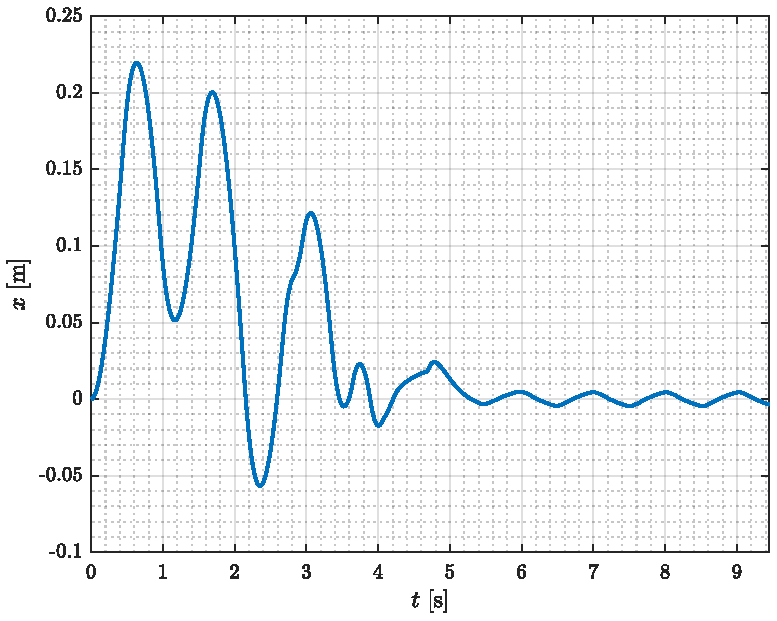
\includegraphics[width=.4\textwidth]{figures/x_swingAndCatch}
  }  
\end{figure}
%
The needed actuation signal is seen in \autoref{fig:ia_swingAndCatch} and though some peaks occur, the RMS stays below the rated continuous current limit of the motor.%The peak at \SI{5}{s} is narrow compared to that in \autoref{fig:ia_slidingMode} since the swing-up controller provides some entry velocity at the catch angle.
%
\begin{figure}[H]
  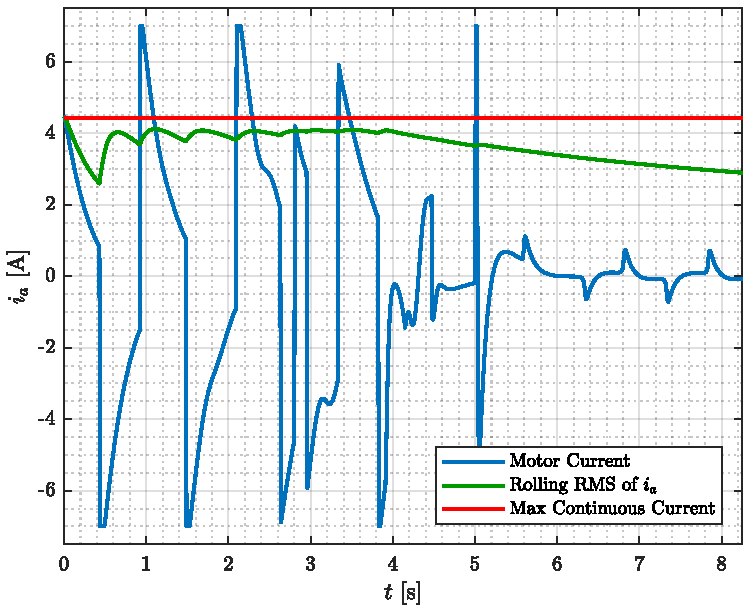
\includegraphics[width=.42\textwidth]{figures/ia_swingAndCatch}
  \caption{Control signal from the simulation in \autoref{fig:theta_swingAndCatch} and \ref{fig:x_swingAndCatch}. Again large peaks occur in the armature current, however, only for short durations and with the RMS staying below the rated continuous current limit.}
  \label{fig:ia_swingAndCatch}
\end{figure}
%
The system was first transformed into \textit{regular form} after which the reduced order system was stabilized using linearization and linear state feedback. Some small oscillations were observed in the nonlinear simulation of the controlled reduced order system. The sliding mode design was proceeded from there based on Lyapunov stability criteria, and the final control law was simulated stabilizing the system also in concert with the swing-up controller.\\
This concludes the stabilization design and carries into the final two chapters of \textit{Part 1} where considerations in implementation are presented along with the final test results from the cart pendulum system setup.
%x
%xDot
%xDotDot
%theta
%thetaDot
%thetaDotDot
%ia
%phase
%Edelta
%ani